\newpage
\subsection{Mechanical Design} \label{Mechanical_Design}
\label{sec:mechanical-design}

\subsubsection{Structure}
\label{sec:4.4.1}
The experiment itself has only two components that are placed inside the Gondola. Firstly, the electronic box and then the gimbal on which the telescope is mounted. We require the gimbal to be placed at the edge of the Gondola so that  we will be able to perform rotating mechanism that pops the telescope out of the gondola while operation.

\begin{figure}[H]
    \centering
	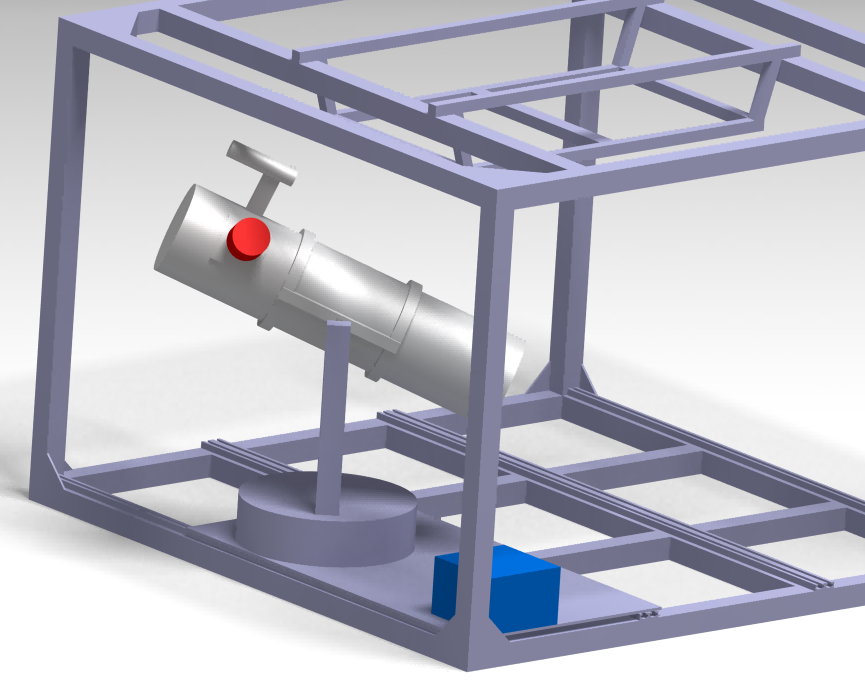
\includegraphics[scale=1.2]{4-experiment-design/img/mechanical/Assembly_3.png}
	\caption{Gimbal structure}
\end{figure}
\subsubsection{Electronic box}
\label{sec:4.4.2}
The electronic box has a dimension 10x10x10 cm which is placed directly inside the gondola. It is estimated to weigh 1.5 kg. The box is made of aluminium side plates with a thick layer of styrofoam placed on the inside of the aluminium plates which protects the electronics. The box has rubber cusion feet that acts as a shock absorber and also thermal insulator from the gondola.

\subsubsection{Gimbal}
\label {sec:4.4.3}
We intend to use a three axis gimbal so we have a maximum field of view. We use CFRP to manufacture the gimbal. The gimbal along with telescope is estimated to weigh around 10kg.



\subsubsection{Fixing interface}
\label {sec:4.4.5}
The telescope itself has certain fixture points. So,we make the gimbal with matching fixture points. The gimbal is directly fixed on the gondola. The gimbal along with the fixing points will first be tested with Finite Element Analysis (FEA) in order to ensure that the whole structure can withstand the loads indicated in the BEXUS manual. 